\documentclass[11pt,letterpaper]{article}
\usepackage{fullpage}

\usepackage[utf8]{inputenc} % allow utf-8 input
\usepackage{hyperref}       % hyperlinks
\usepackage{url}            % simple URL typesetting
\usepackage{booktabs}       % professional-quality tables
\usepackage{amsfonts}       % blackboard math symbols
\usepackage{nicefrac}       % compact symbols for 1/2, etc.
\usepackage{microtype}      % microtypography
\usepackage{amssymb}
\usepackage{natbib}
%% The amsthm package provides extended theorem environments
\usepackage{amsthm}
\usepackage{float}
\usepackage{sgame, tikz} % Game theory packages
\usepackage{caption} 
\usepackage{algorithm,algpseudocode}
\usepackage{makecell}
 \usepackage{multirow}
 \usepackage{graphicx}
             
\graphicspath{{../results}}
\begin{document} 

\title{Supplemental Material}
\date{}
\maketitle

\appendix
\section{Additional Isolation Performance Plots}

In this section we present the additional mean reputation graphs that were omitted from the main text. Additionally, we provide graphs of the smoothed mean instantaneous reward for each of the family of instances that we consider.

\begin{center}
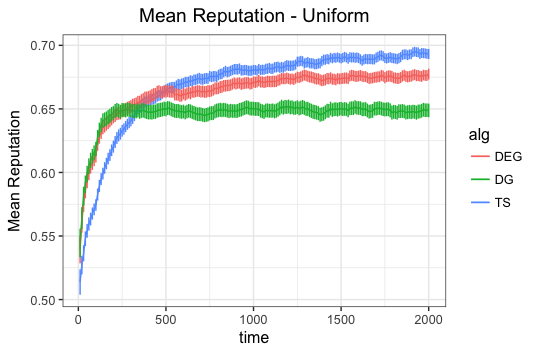
\includegraphics[scale=0.5]{figures/uniform_mean} \\
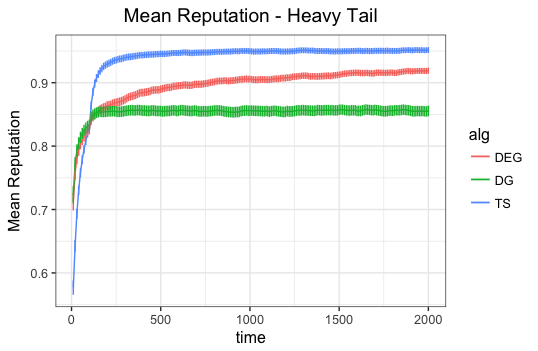
\includegraphics[scale=0.5]{figures/ht_mean} \\
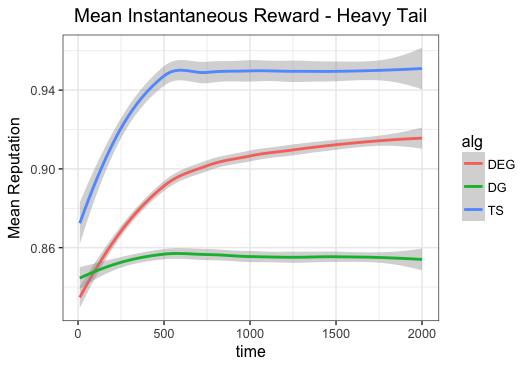
\includegraphics[scale=0.5]{figures/mean_inst_reward_ht} \\
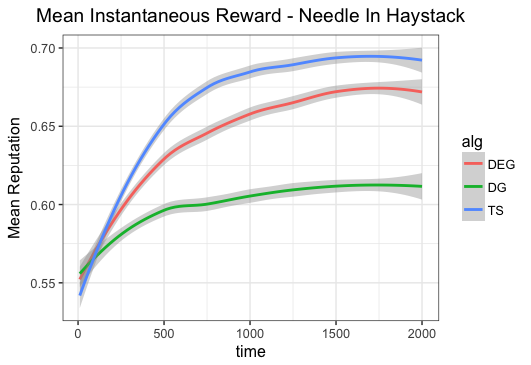
\includegraphics[scale=0.5]{figures/mean_inst_reward_nih} \\
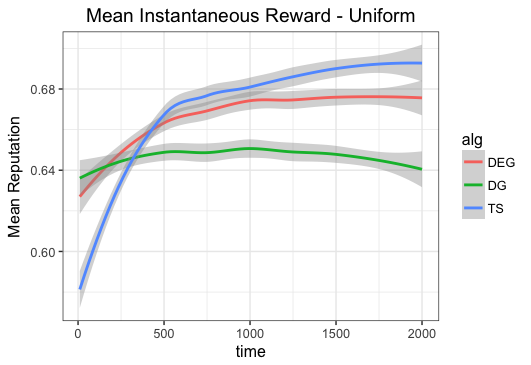
\includegraphics[scale=0.5]{figures/mean_inst_reward_uniform}
\end{center}

\pagebreak
\section{Reversal between Mean Reputation and Relative Reputation}

In this section we present the results in isolation and in competition over the ``Heavy Tail" prior discussed in the text for $K = 3$. We demonstrate evidence that $DEG > DG$ according to the mean reputation metric but that $DG > DEG$ according to the relative reputation proportion statistic and in the competition game. As shown in the text, the same results also hold for $K = 10$ for the warm starts that we consider.

\begin{center}
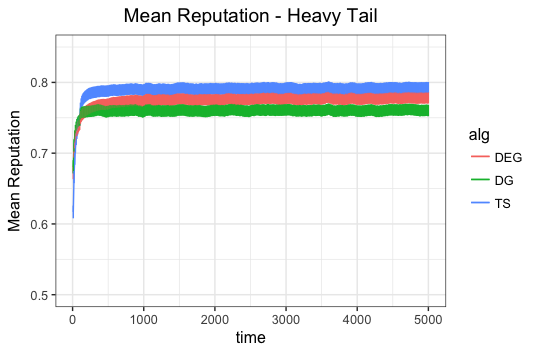
\includegraphics[scale=0.5]{figures/mean_ht_3_arms} \\
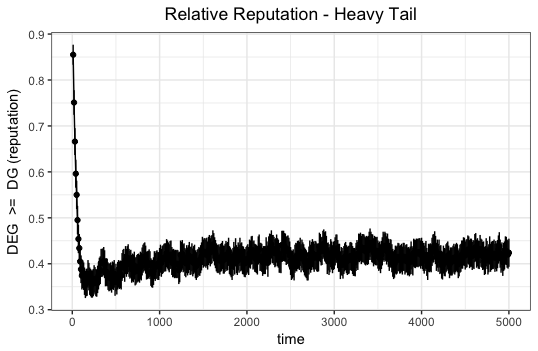
\includegraphics[scale=0.5]{figures/rel_rep_ht_3_arms}
\end{center}

\begin{table}[H]
\centering
\caption{Duopoly Experiment Heavy Tail K=3, t=5000} 
\begin{tabular}{rlll}
  \hline
 & k = 20 & k = 250 & k = 500 \\ 
  \hline
TS vs DG & \makecell{\textbf{0.4} $\pm$0.02\\ eeog \\ avg: 770\\ med: 0} & \makecell{\textbf{0.59} $\pm$0.01\\ eeog \\ avg: 2700\\ med: 2979.5} & \makecell{\textbf{0.6} $\pm$0.01\\ eeog \\ avg: 2700\\ med: 3018} \\ 
  TS vs DEG & \makecell{\textbf{0.46} $\pm$0.02\\ eeog \\ avg: 830\\ med: 0} & \makecell{\textbf{0.73} $\pm$0.01\\ eeog \\ avg: 2500\\ med: 2576.5} & \makecell{\textbf{0.72} $\pm$0.01\\ eeog \\ avg: 2700\\ med: 2862} \\ 
  DG vs DEG & \makecell{\textbf{0.61} $\pm$0.01\\ eeog \\ avg: 1400\\ med: 556} & \makecell{\textbf{0.61} $\pm$0.01\\ eeog \\ avg: 2400\\ med: 2538.5} & \makecell{\textbf{0.6} $\pm$0.01\\ eeog \\ avg: 2400\\ med: 2587.5} \\ 
   \hline
\end{tabular}
\end{table}

\section{Additional Permanent Duopoly Experiments}

We present all of the results for the permanent duopoly experiments across the family of instances that we consider. The results displayed in the table are the same contain the same information as those in the text and are the average over $N = 1000$ simulations.

\begin{table}[H]
\centering
\caption{Duopoly Experiment Needle In Haystack} 
\begin{tabular}{rlll}
  \hline
 & $T_0$ = 20 & $T_0$ = 250 & $T_0$ = 500 \\ 
  \hline
TS vs DG & \makecell{\textbf{0.64} $\pm$0.03\\ eeog \\ avg: 200\\ med: 27} & \makecell{\textbf{0.6} $\pm$0.03\\ eeog \\ avg: 370\\ med: 0} & \makecell{\textbf{0.64} $\pm$0.03\\ eeog \\ avg: 580\\ med: 121.5} \\ 
  TS vs DEG & \makecell{\textbf{0.57} $\pm$0.03\\ eeog \\ avg: 150\\ med: 14} & \makecell{\textbf{0.52} $\pm$0.03\\ eeog \\ avg: 460\\ med: 78.5} & \makecell{\textbf{0.56} $\pm$0.02\\ eeog \\ avg: 740\\ med: 627.5} \\ 
  DG vs DEG & \makecell{\textbf{0.46} $\pm$0.03\\ eeog \\ avg: 340\\ med: 128.5} & \makecell{\textbf{0.42} $\pm$0.02\\ eeog \\ avg: 650\\ med: 408} & \makecell{\textbf{0.42} $\pm$0.02\\ eeog \\ avg: 690\\ med: 466.5} \\ 
   \hline
\end{tabular}
\end{table}
% latex table generated in R 3.4.0 by xtable 1.8-2 package
% Sat Sep  1 12:45:03 2018
\begin{table}[H]
\centering
\caption{Duopoly Experiment Heavy Tail} 
\begin{tabular}{rlll}
  \hline
 & $T_0$ = 20 & $T_0$ = 250 & $T_0$ = 500 \\ 
  \hline
TS vs DG & \makecell{\textbf{0.29} $\pm$0.03\\ eeog \\ avg: 55\\ med: 0} & \makecell{\textbf{0.72} $\pm$0.02\\ eeog \\ avg: 570\\ med: 0} & \makecell{\textbf{0.76} $\pm$0.02\\ eeog \\ avg: 620\\ med: 98.5} \\ 
  TS vs DEG & \makecell{\textbf{0.3} $\pm$0.03\\ eeog \\ avg: 37\\ med: 0} & \makecell{\textbf{0.88} $\pm$0.01\\ eeog \\ avg: 480\\ med: 0} & \makecell{\textbf{0.9} $\pm$0.01\\ eeog \\ avg: 570\\ med: 113.5} \\ 
  DG vs DEG & \makecell{\textbf{0.62} $\pm$0.03\\ eeog \\ avg: 410\\ med: 7} & \makecell{\textbf{0.6} $\pm$0.02\\ eeog \\ avg: 790\\ med: 762} & \makecell{\textbf{0.57} $\pm$0.03\\ eeog \\ avg: 730\\ med: 608} \\ 
   \hline
\end{tabular}
\end{table}
% latex table generated in R 3.4.0 by xtable 1.8-2 package
% Sat Sep  1 12:45:03 2018
\begin{table}[H]
\centering
\caption{Duopoly Experiment Uniform} 
\begin{tabular}{rlll}
  \hline
 & $T_0$ = 20 & $T_0$ = 250 & $T_0$ = 500 \\ 
  \hline
TS vs DG & \makecell{\textbf{0.46} $\pm$0.03\\ eeog \\ avg: 230\\ med: 0} & \makecell{\textbf{0.52} $\pm$0.02\\ eeog \\ avg: 800\\ med: 754} & \makecell{\textbf{0.6} $\pm$0.02\\ eeog \\ avg: 910\\ med: 906.5} \\ 
  TS vs DEG & \makecell{\textbf{0.41} $\pm$0.03\\ eeog \\ avg: 180\\ med: 0} & \makecell{\textbf{0.51} $\pm$0.02\\ eeog \\ avg: 810\\ med: 734} & \makecell{\textbf{0.55} $\pm$0.02\\ eeog \\ avg: 970\\ med: 987} \\ 
  DG vs DEG & \makecell{\textbf{0.51} $\pm$0.03\\ eeog \\ avg: 470\\ med: 57.5} & \makecell{\textbf{0.48} $\pm$0.02\\ eeog \\ avg: 1000\\ med: 1088} & \makecell{\textbf{0.45} $\pm$0.02\\ eeog \\ avg: 1000\\ med: 1142} \\ 
   \hline
\end{tabular}
\end{table}

\newpage

\section{Additional Temporary Monopoly Experiments}

We present results for the temporary monopoly experiment across the family of instances that we consider for varying values of $X$. These results confirm the claim in the text that, for sufficiently large $X$, Thompson Sampling is preferred over all other algorithms for the incumbent. However, it also shows that, for smaller values of $X$ it is not necessarily the case that Thompson Sampling is the preferred algorithm. We provide many different parameterizations in order to check the robustness of the results. The results displayed in the table are the same contain the same information as those in the text and are the average over $N = 1000$ simulations.

\subsection*{Heavy Tail Prior}
\begin{table}[H]
\centering
\caption{Temporary Monopoly Experiment Heavy Tail X = 50} 
\begin{tabular}{rlll}
\hline
\multicolumn{4}{c}{Incumbent Algorithm}\\
\multirow{12}{0.6in}{\rotatebox{90}{Entrant Algorithm}} \\
  \hline
 & TS & DEG &  DG \\ 
  \hline
TS & \makecell{\textbf{0.054} $\pm$0.01\\Var:0.05\\ES:100\%} & \makecell{\textbf{0.16} $\pm$0.02\\Var:0.1\\ES:97\%} & \makecell{\textbf{0.18} $\pm$0.02\\Var:0.1\\ES:95\%} \\ 
  DEG & \makecell{\textbf{0.33} $\pm$0.03\\Var:0.2\\ES:95\%} & \makecell{\textbf{0.31} $\pm$0.02\\Var:0.2\\ES:76\%} & \makecell{\textbf{0.26} $\pm$0.02\\Var:0.1\\ES:79\%} \\ 
   DG & \makecell{\textbf{0.39} $\pm$0.03\\Var:0.2\\ES:95\%} & \makecell{\textbf{0.41} $\pm$0.03\\Var:0.2\\ES:76\%} & \makecell{\textbf{0.33} $\pm$0.02\\Var:0.2\\ES:67\%} \\ 
   \hline
\end{tabular}
\end{table}
\begin{table}[H]
\centering
\caption{Temporary Monopoly Experiment Heavy Tail X = 200} 
\begin{tabular}{rlll}
\hline
\multicolumn{4}{c}{Incumbent Algorithm}\\
\multirow{12}{0.6in}{\rotatebox{90}{Entrant Algorithm}} \\
  \hline
 & TS & DEG &  DG \\ 
  \hline
TS & \makecell{\textbf{0.003} $\pm$0.003\\Var:0.002\\ES:100\%} & \makecell{\textbf{0.083} $\pm$0.02\\Var:0.07\\ES:97\%} & \makecell{\textbf{0.17} $\pm$0.02\\Var:0.1\\ES:95\%} \\ 
  DEG & \makecell{\textbf{0.045} $\pm$0.01\\Var:0.03\\ES:92\%} & \makecell{\textbf{0.25} $\pm$0.02\\Var:0.1\\ES:75\%} & \makecell{\textbf{0.23} $\pm$0.02\\Var:0.1\\ES:78\%} \\ 
   DG & \makecell{\textbf{0.12} $\pm$0.02\\Var:0.08\\ES:88\%} & \makecell{\textbf{0.36} $\pm$0.03\\Var:0.2\\ES:76\%} & \makecell{\textbf{0.3} $\pm$0.02\\Var:0.1\\ES:64\%} \\ 
   \hline
\end{tabular}
\end{table}

\begin{table}[H]
\centering
\caption{Temporary Monopoly Experiment Heavy Tail X = 300} 
\begin{tabular}{rlll}
\hline
\multicolumn{4}{c}{Incumbent Algorithm}\\
\multirow{12}{0.6in}{\rotatebox{90}{Entrant Algorithm}} \\
  \hline
 & TS & DEG &  DG \\ 
  \hline
TS & \makecell{\textbf{0.0017} $\pm$0.002\\Var:0.001\\ES:100\%} & \makecell{\textbf{0.059} $\pm$0.01\\Var:0.05\\ES:99\%} & \makecell{\textbf{0.16} $\pm$0.02\\Var:0.1\\ES:95\%} \\ 
  DEG & \makecell{\textbf{0.029} $\pm$0.007\\Var:0.01\\ES:93\%} & \makecell{\textbf{0.23} $\pm$0.02\\Var:0.1\\ES:74\%} & \makecell{\textbf{0.23} $\pm$0.02\\Var:0.1\\ES:78\%} \\ 
   DG & \makecell{\textbf{0.097} $\pm$0.02\\Var:0.06\\ES:89\%} & \makecell{\textbf{0.34} $\pm$0.03\\Var:0.2\\ES:76\%} & \makecell{\textbf{0.29} $\pm$0.02\\Var:0.1\\ES:66\%} \\ 
   \hline
\end{tabular}
\end{table}

\begin{table}[H]
\centering
\caption{Temporary Monopoly Experiment Heavy Tail X = 500} 
\begin{tabular}{rlll}
\hline
\multicolumn{4}{c}{Incumbent Algorithm}\\
\multirow{12}{0.6in}{\rotatebox{90}{Entrant Algorithm}} \\
  \hline
 & TS & DEG &  DG \\ 
  \hline
TS & \makecell{\textbf{0.002} $\pm$0.003\\Var:0.002\\ES:100\%} & \makecell{\textbf{0.043} $\pm$0.01\\Var:0.04\\ES:98\%} & \makecell{\textbf{0.16} $\pm$0.02\\Var:0.1\\ES:94\%} \\ 
  DEG & \makecell{\textbf{0.03} $\pm$0.007\\Var:0.01\\ES:92\%} & \makecell{\textbf{0.21} $\pm$0.02\\Var:0.1\\ES:76\%} & \makecell{\textbf{0.24} $\pm$0.02\\Var:0.1\\ES:78\%} \\ 
   DG & \makecell{\textbf{0.091} $\pm$0.01\\Var:0.05\\ES:87\%} & \makecell{\textbf{0.32} $\pm$0.03\\Var:0.2\\ES:78\%} & \makecell{\textbf{0.3} $\pm$0.02\\Var:0.1\\ES:65\%} \\ 
   \hline
\end{tabular}
\end{table}

\subsection*{Needle In Haystack Prior}

% latex table generated in R 3.4.0 by xtable 1.8-2 package
% Sat Aug 25 17:05:40 2018
\begin{table}[H]
\centering
\caption{Temporary Monopoly Experiment Needle In Haystack X = 50} 
\begin{tabular}{rlll}
\hline
\multicolumn{4}{c}{Incumbent Algorithm}\\
\multirow{12}{0.6in}{\rotatebox{90}{Entrant Algorithm}} \\
  \hline
 & TS & DEG &  DG \\ 
  \hline
TS & \makecell{\textbf{0.34} $\pm$0.03\\Var:0.2\\ES:92\%} & \makecell{\textbf{0.4} $\pm$0.03\\Var:0.2\\ES:90\%} & \makecell{\textbf{0.48} $\pm$0.03\\Var:0.2\\ES:85\%} \\ 
  DEG & \makecell{\textbf{0.22} $\pm$0.02\\Var:0.1\\ES:93\%} & \makecell{\textbf{0.34} $\pm$0.03\\Var:0.2\\ES:83\%} & \makecell{\textbf{0.42} $\pm$0.03\\Var:0.2\\ES:75\%} \\ 
   DG & \makecell{\textbf{0.18} $\pm$0.02\\Var:0.1\\ES:89\%} & \makecell{\textbf{0.28} $\pm$0.02\\Var:0.2\\ES:78\%} & \makecell{\textbf{0.37} $\pm$0.03\\Var:0.2\\ES:70\%} \\ 
   \hline
\end{tabular}
\end{table}

% latex table generated in R 3.4.0 by xtable 1.8-2 package
% Sat Aug 25 17:07:02 2018
\begin{table}[H]
\centering
\caption{Temporary Monopoly Experiment Needle In Haystack X = 200} 
\begin{tabular}{rlll}
\hline
\multicolumn{4}{c}{Incumbent Algorithm}\\
\multirow{12}{0.6in}{\rotatebox{90}{Entrant Algorithm}} \\
  \hline
 & TS & DEG &  DG \\ 
  \hline
TS & \makecell{\textbf{0.17} $\pm$0.02\\Var:0.1\\ES:95\%} & \makecell{\textbf{0.31} $\pm$0.03\\Var:0.2\\ES:90\%} & \makecell{\textbf{0.41} $\pm$0.03\\Var:0.2\\ES:86\%} \\ 
  DEG & \makecell{\textbf{0.13} $\pm$0.02\\Var:0.1\\ES:95\%} & \makecell{\textbf{0.26} $\pm$0.02\\Var:0.2\\ES:85\%} & \makecell{\textbf{0.36} $\pm$0.03\\Var:0.2\\ES:78\%} \\ 
   DG & \makecell{\textbf{0.093} $\pm$0.02\\Var:0.07\\ES:94\%} & \makecell{\textbf{0.23} $\pm$0.02\\Var:0.1\\ES:83\%} & \makecell{\textbf{0.33} $\pm$0.03\\Var:0.2\\ES:74\%} \\ 
   \hline
\end{tabular}
\end{table}

% latex table generated in R 3.4.0 by xtable 1.8-2 package
% Sat Aug 25 17:07:42 2018
\begin{table}[H]
\centering
\caption{Temporary Monopoly Experiment Needle In Haystack X = 300} 
\begin{tabular}{rlll}
\hline
\multicolumn{4}{c}{Incumbent Algorithm}\\
\multirow{12}{0.6in}{\rotatebox{90}{Entrant Algorithm}} \\
  \hline
 & TS & DEG &  DG \\ 
  \hline
TS & \makecell{\textbf{0.1} $\pm$0.02\\Var:0.07\\ES:95\%} & \makecell{\textbf{0.28} $\pm$0.03\\Var:0.2\\ES:91\%} & \makecell{\textbf{0.39} $\pm$0.03\\Var:0.2\\ES:87\%} \\ 
  DEG & \makecell{\textbf{0.089} $\pm$0.02\\Var:0.06\\ES:94\%} & \makecell{\textbf{0.23} $\pm$0.02\\Var:0.2\\ES:88\%} & \makecell{\textbf{0.36} $\pm$0.03\\Var:0.2\\ES:80\%} \\ 
   DG & \makecell{\textbf{0.05} $\pm$0.01\\Var:0.03\\ES:96\%} & \makecell{\textbf{0.21} $\pm$0.02\\Var:0.1\\ES:83\%} & \makecell{\textbf{0.33} $\pm$0.03\\Var:0.2\\ES:74\%} \\ 
   \hline
\end{tabular}
\end{table}

% latex table generated in R 3.4.0 by xtable 1.8-2 package
% Sun Aug 26 09:19:46 2018
\begin{table}[H]
\centering
\caption{Temporary Monopoly Experiment Needle In Haystack X = 500} 
\begin{tabular}{rlll}
\hline
\multicolumn{4}{c}{Incumbent Algorithm}\\
\multirow{12}{0.6in}{\rotatebox{90}{Entrant Algorithm}} \\
  \hline
 & TS & DEG &  DG \\ 
  \hline
TS & \makecell{\textbf{0.053} $\pm$0.01\\Var:0.04\\ES:95\%} & \makecell{\textbf{0.23} $\pm$0.02\\Var:0.2\\ES:92\%} & \makecell{\textbf{0.37} $\pm$0.03\\Var:0.2\\ES:88\%} \\ 
  DEG & \makecell{\textbf{0.051} $\pm$0.01\\Var:0.04\\ES:97\%} & \makecell{\textbf{0.2} $\pm$0.02\\Var:0.1\\ES:89\%} & \makecell{\textbf{0.33} $\pm$0.03\\Var:0.2\\ES:80\%} \\ 
   DG & \makecell{\textbf{0.031} $\pm$0.009\\Var:0.02\\ES:98\%} & \makecell{\textbf{0.18} $\pm$0.02\\Var:0.1\\ES:88\%} & \makecell{\textbf{0.31} $\pm$0.02\\Var:0.2\\ES:76\%} \\ 
   \hline
\end{tabular}
\end{table}


\subsection*{Uniform Prior}

% latex table generated in R 3.4.0 by xtable 1.8-2 package
% Sat Aug 25 17:05:41 2018
\begin{table}[H]
\centering
\caption{Temporary Monopoly Experiment Uniform X = 50} 
\begin{tabular}{rlll}
\hline
\multicolumn{4}{c}{Incumbent Algorithm}\\
\multirow{12}{0.6in}{\rotatebox{90}{Entrant Algorithm}} \\
  \hline
 & TS & DEG &  DG \\ 
  \hline
TS & \makecell{\textbf{0.27} $\pm$0.03\\Var:0.2\\ES:91\%} & \makecell{\textbf{0.21} $\pm$0.02\\Var:0.1\\ES:88\%} & \makecell{\textbf{0.26} $\pm$0.02\\Var:0.2\\ES:83\%} \\ 
  DEG & \makecell{\textbf{0.39} $\pm$0.03\\Var:0.2\\ES:84\%} & \makecell{\textbf{0.3} $\pm$0.03\\Var:0.2\\ES:80\%} & \makecell{\textbf{0.34} $\pm$0.03\\Var:0.2\\ES:73\%} \\ 
   DG & \makecell{\textbf{0.39} $\pm$0.03\\Var:0.2\\ES:85\%} & \makecell{\textbf{0.31} $\pm$0.02\\Var:0.2\\ES:74\%} & \makecell{\textbf{0.33} $\pm$0.02\\Var:0.2\\ES:70\%} \\ 
   \hline
\end{tabular}
\end{table}

% latex table generated in R 3.4.0 by xtable 1.8-2 package
% Sat Aug 25 17:08:22 2018
\begin{table}[H]
\centering
\caption{Temporary Monopoly Experiment Uniform X = 200} 
\begin{tabular}{rlll}
\hline
\multicolumn{4}{c}{Incumbent Algorithm}\\
\multirow{12}{0.6in}{\rotatebox{90}{Entrant Algorithm}} \\
\hline
 & TS & DEG &  DG \\ 
  \hline
TS & \makecell{\textbf{0.12} $\pm$0.02\\Var:0.08\\ES:89\%} & \makecell{\textbf{0.16} $\pm$0.02\\Var:0.1\\ES:87\%} & \makecell{\textbf{0.2} $\pm$0.02\\Var:0.1\\ES:84\%} \\ 
  DEG & \makecell{\textbf{0.25} $\pm$0.02\\Var:0.1\\ES:81\%} & \makecell{\textbf{0.24} $\pm$0.02\\Var:0.1\\ES:77\%} & \makecell{\textbf{0.29} $\pm$0.02\\Var:0.1\\ES:71\%} \\ 
   DG & \makecell{\textbf{0.23} $\pm$0.02\\Var:0.1\\ES:80\%} & \makecell{\textbf{0.24} $\pm$0.02\\Var:0.1\\ES:76\%} & \makecell{\textbf{0.29} $\pm$0.02\\Var:0.1\\ES:69\%} \\ 
   \hline
\end{tabular}
\end{table}

% latex table generated in R 3.4.0 by xtable 1.8-2 package
% Sat Aug 25 17:07:43 2018
\begin{table}[H]
\centering
\caption{Temporary Monopoly Experiment Uniform X = 300} 
\begin{tabular}{rlll}
\hline
\multicolumn{4}{c}{Incumbent Algorithm}\\
\multirow{12}{0.6in}{\rotatebox{90}{Entrant Algorithm}} \\
  \hline
 & TS & DEG &  DG \\ 
  \hline
TS & \makecell{\textbf{0.094} $\pm$0.02\\Var:0.06\\ES:90\%} & \makecell{\textbf{0.15} $\pm$0.02\\Var:0.1\\ES:86\%} & \makecell{\textbf{0.2} $\pm$0.02\\Var:0.1\\ES:85\%} \\ 
  DEG & \makecell{\textbf{0.2} $\pm$0.02\\Var:0.1\\ES:80\%} & \makecell{\textbf{0.23} $\pm$0.02\\Var:0.1\\ES:74\%} & \makecell{\textbf{0.29} $\pm$0.02\\Var:0.1\\ES:70\%} \\ 
   DG & \makecell{\textbf{0.21} $\pm$0.02\\Var:0.1\\ES:79\%} & \makecell{\textbf{0.23} $\pm$0.02\\Var:0.1\\ES:74\%} & \makecell{\textbf{0.29} $\pm$0.02\\Var:0.1\\ES:70\%} \\ 
   \hline
\end{tabular}
\end{table}

\begin{table}[H]
\centering
\caption{Temporary Monopoly Experiment Uniform X = 500} 
\begin{tabular}{rlll}
\hline
\multicolumn{4}{c}{Incumbent Algorithm}\\
\multirow{12}{0.6in}{\rotatebox{90}{Entrant Algorithm}} \\
  \hline
 & TS & DEG &  DG \\ 
  \hline
TS & \makecell{\textbf{0.061} $\pm$0.01\\Var:0.03\\ES:91\%} & \makecell{\textbf{0.12} $\pm$0.02\\Var:0.08\\ES:88\%} & \makecell{\textbf{0.2} $\pm$0.02\\Var:0.1\\ES:84\%} \\ 
  DEG & \makecell{\textbf{0.17} $\pm$0.02\\Var:0.09\\ES:79\%} & \makecell{\textbf{0.21} $\pm$0.02\\Var:0.1\\ES:75\%} & \makecell{\textbf{0.29} $\pm$0.02\\Var:0.1\\ES:73\%} \\ 
   DG & \makecell{\textbf{0.18} $\pm$0.02\\Var:0.1\\ES:78\%} & \makecell{\textbf{0.22} $\pm$0.02\\Var:0.1\\ES:75\%} & \makecell{\textbf{0.29} $\pm$0.02\\Var:0.1\\ES:70\%} \\ 
   \hline
\end{tabular}
\end{table}

\section{Reputation and Information Erased Experiment}

This section contains the results on all of the family of instances for the reputation and information erased experiment discussed in the ``Data and Reputation as Barriers to Entry" section of the paper.

\begin{table}[H]
\centering
\caption{Reputation Erased Experiment Heavy Tail} 
\begin{tabular}{rlll}
\hline
\multicolumn{4}{c}{Incumbent Algorithm}\\
\multirow{12}{0.6in}{\rotatebox{90}{Entrant Algorithm}} \\
  \hline
 & TS & DEG &  DG \\ 
  \hline
TS & \makecell{\textbf{ 0.0096 } $\pm$ 0.006 \\Var: 0.009 \\ ES: 100 \%} & \makecell{\textbf{ 0.11 } $\pm$ 0.02 \\Var: 0.09 \\ ES: 98 \%} & \makecell{\textbf{ 0.18 } $\pm$ 0.02 \\Var: 0.1 \\ ES: 95 \%} \\ 
  DEG & \makecell{\textbf{ 0.073 } $\pm$ 0.01 \\Var: 0.05 \\ ES: 93 \%} & \makecell{\textbf{ 0.29 } $\pm$ 0.02 \\Var: 0.2 \\ ES: 78 \%} & \makecell{\textbf{ 0.25 } $\pm$ 0.02 \\Var: 0.1 \\ ES: 79 \%} \\ 
   DG & \makecell{\textbf{ 0.15 } $\pm$ 0.02 \\Var: 0.1 \\ ES: 89 \%} & \makecell{\textbf{ 0.39 } $\pm$ 0.03 \\Var: 0.2 \\ ES: 78 \%} & \makecell{\textbf{ 0.33 } $\pm$ 0.02 \\Var: 0.2 \\ ES: 66 \%} \\ 
   \hline
\end{tabular}
\end{table}

\begin{table}[H]
\centering
\caption{Information Erased Experiment Heavy Tail} 
\begin{tabular}{rlll}
\hline
\multicolumn{4}{c}{Incumbent Algorithm}\\
\multirow{12}{0.6in}{\rotatebox{90}{Entrant Algorithm}} \\
  \hline
 & TS & DEG &  DG \\ 
  \hline
TS & \makecell{\textbf{ 0.021 } $\pm$ 0.009 \\Var: 0.02 \\ ES: 100 \%} & \makecell{\textbf{ 0.16 } $\pm$ 0.02 \\Var: 0.1 \\ ES: 97 \%} & \makecell{\textbf{ 0.21 } $\pm$ 0.02 \\Var: 0.2 \\ ES: 95 \%} \\ 
  DEG & \makecell{\textbf{ 0.26 } $\pm$ 0.03 \\Var: 0.2 \\ ES: 95 \%} & \makecell{\textbf{ 0.3 } $\pm$ 0.02 \\Var: 0.2 \\ ES: 74 \%} & \makecell{\textbf{ 0.26 } $\pm$ 0.02 \\Var: 0.1 \\ ES: 76 \%} \\ 
   DG & \makecell{\textbf{ 0.34 } $\pm$ 0.03 \\Var: 0.2 \\ ES: 94 \%} & \makecell{\textbf{ 0.4 } $\pm$ 0.03 \\Var: 0.2 \\ ES: 74 \%} & \makecell{\textbf{ 0.33 } $\pm$ 0.02 \\Var: 0.1 \\ ES: 58 \%} \\ 
   \hline
\end{tabular}
\end{table}


% latex table generated in R 3.4.0 by xtable 1.8-2 package
% Sun Aug 26 09:51:12 2018
\begin{table}[H]
\centering
\caption{Reputation Erased Experiment Needle In Haystack} 
\begin{tabular}{rlll}
\hline
\multicolumn{4}{c}{Incumbent Algorithm}\\
\multirow{12}{0.6in}{\rotatebox{90}{Entrant Algorithm}} \\
  \hline
 & TS & DEG &  DG \\ 
  \hline
TS & \makecell{\textbf{ 0.25 } $\pm$ 0.03 \\Var: 0.2 \\ ES: 96 \%} & \makecell{\textbf{ 0.36 } $\pm$ 0.03 \\Var: 0.2 \\ ES: 93 \%} & \makecell{\textbf{ 0.45 } $\pm$ 0.03 \\Var: 0.2 \\ ES: 89 \%} \\ 
  DEG & \makecell{\textbf{ 0.21 } $\pm$ 0.02 \\Var: 0.1 \\ ES: 93 \%} & \makecell{\textbf{ 0.32 } $\pm$ 0.03 \\Var: 0.2 \\ ES: 89 \%} & \makecell{\textbf{ 0.41 } $\pm$ 0.03 \\Var: 0.2 \\ ES: 83 \%} \\ 
   DG & \makecell{\textbf{ 0.18 } $\pm$ 0.02 \\Var: 0.1 \\ ES: 92 \%} & \makecell{\textbf{ 0.29 } $\pm$ 0.03 \\Var: 0.2 \\ ES: 86 \%} & \makecell{\textbf{ 0.4 } $\pm$ 0.03 \\Var: 0.2 \\ ES: 78 \%} \\ 
   \hline
\end{tabular}
\end{table}

\begin{table}[H]
\centering
\caption{Information Erased Experiment Needle In Haystack}
\begin{tabular}{rlll}
\hline
\multicolumn{4}{c}{Incumbent Algorithm}\\
\multirow{12}{0.6in}{\rotatebox{90}{Entrant Algorithm}} \\
  \hline
 & TS & DEG &  DG \\ 
  \hline
TS & \makecell{\textbf{ 0.35 } $\pm$ 0.03 \\Var: 0.2 \\ ES: 93 \%} & \makecell{\textbf{ 0.43 } $\pm$ 0.03 \\Var: 0.2 \\ ES: 88 \%} & \makecell{\textbf{ 0.52 } $\pm$ 0.03 \\Var: 0.2 \\ ES: 82 \%} \\ 
  DEG & \makecell{\textbf{ 0.26 } $\pm$ 0.03 \\Var: 0.2 \\ ES: 90 \%} & \makecell{\textbf{ 0.36 } $\pm$ 0.03 \\Var: 0.2 \\ ES: 80 \%} & \makecell{\textbf{ 0.43 } $\pm$ 0.03 \\Var: 0.2 \\ ES: 71 \%} \\ 
   DG & \makecell{\textbf{ 0.19 } $\pm$ 0.02 \\Var: 0.1 \\ ES: 85 \%} & \makecell{\textbf{ 0.3 } $\pm$ 0.02 \\Var: 0.1 \\ ES: 73 \%} & \makecell{\textbf{ 0.36 } $\pm$ 0.02 \\Var: 0.2 \\ ES: 64 \%} \\ 
   \hline
\end{tabular}
\end{table}

% latex table generated in R 3.4.0 by xtable 1.8-2 package
% Sun Aug 26 09:51:13 2018
\begin{table}[H]
\centering
\caption{Reputation Erased Experiment Uniform} 
\begin{tabular}{rlll}
\hline
\multicolumn{4}{c}{Incumbent Algorithm}\\
\multirow{12}{0.6in}{\rotatebox{90}{Entrant Algorithm}} \\
  \hline
 & TS & DEG &  DG \\ 
  \hline
TS & \makecell{\textbf{ 0.2 } $\pm$ 0.02 \\Var: 0.1 \\ ES: 89 \%} & \makecell{\textbf{ 0.22 } $\pm$ 0.02 \\Var: 0.1 \\ ES: 88 \%} & \makecell{\textbf{ 0.27 } $\pm$ 0.03 \\Var: 0.2 \\ ES: 87 \%} \\ 
  DEG & \makecell{\textbf{ 0.33 } $\pm$ 0.03 \\Var: 0.2 \\ ES: 81 \%} & \makecell{\textbf{ 0.32 } $\pm$ 0.03 \\Var: 0.2 \\ ES: 79 \%} & \makecell{\textbf{ 0.35 } $\pm$ 0.03 \\Var: 0.2 \\ ES: 75 \%} \\ 
   DG & \makecell{\textbf{ 0.32 } $\pm$ 0.03 \\Var: 0.2 \\ ES: 80 \%} & \makecell{\textbf{ 0.31 } $\pm$ 0.03 \\Var: 0.2 \\ ES: 77 \%} & \makecell{\textbf{ 0.35 } $\pm$ 0.03 \\Var: 0.2 \\ ES: 73 \%} \\ 
   \hline
\end{tabular}
\end{table}

\begin{table}[H]
\centering
\caption{Information Erased Experiment Uniform} 
\begin{tabular}{rlll}
\hline
\multicolumn{4}{c}{Incumbent Algorithm}\\
\multirow{12}{0.6in}{\rotatebox{90}{Entrant Algorithm}} \\
  \hline
 & TS & DEG &  DG \\ 
  \hline
TS & \makecell{\textbf{ 0.27 } $\pm$ 0.03 \\Var: 0.2 \\ ES: 91 \%} & \makecell{\textbf{ 0.23 } $\pm$ 0.02 \\Var: 0.1 \\ ES: 87 \%} & \makecell{\textbf{ 0.27 } $\pm$ 0.02 \\Var: 0.2 \\ ES: 84 \%} \\ 
  DEG & \makecell{\textbf{ 0.4 } $\pm$ 0.03 \\Var: 0.2 \\ ES: 86 \%} & \makecell{\textbf{ 0.3 } $\pm$ 0.02 \\Var: 0.2 \\ ES: 72 \%} & \makecell{\textbf{ 0.32 } $\pm$ 0.02 \\Var: 0.2 \\ ES: 69 \%} \\ 
   DG & \makecell{\textbf{ 0.36 } $\pm$ 0.03 \\Var: 0.2 \\ ES: 83 \%} & \makecell{\textbf{ 0.29 } $\pm$ 0.02 \\Var: 0.1 \\ ES: 69 \%} & \makecell{\textbf{ 0.3 } $\pm$ 0.02 \\Var: 0.1 \\ ES: 60 \%} \\ 
   \hline
\end{tabular}
\end{table}


\end{document}